%% ----------------------------------------------------------------
%%? 1st Draft In Progress 2000 words
%% ---------------------------------------------------------------- 
\chapter{Development}
\section{Chosen Techonology Stack}
\subsection{Application Framework: Tauri vs Electron}
Tauri and Electron are the two main frameworks for building native applications using web technologies. They both create an executable than can be run on any operating system. Electron bundles a version of Chromium into the executable, increasing the size of the application compared to Tauri, but resulting in a consistent experience across any OS. Tauri uses the default browser of the operating system, which means it is smaller in size, but more inconsistent. As the application will mainly be tested using Windows machines, this inconsistency is not an issue.

The main difference between Tauri and Electron resides in the backend; Electron is JavaScript-based, whilst Tauri is Rust-based. Due to the type-safety and prior experience in Rust, Tauri is the more optimal choice for the backend. Tauri also integrates with any frontend framework much simpler than Electron does (Electron requires more manual setup). 

Tauri is less widely-used than Electron however, meaning there is less community support. However, Tauri is still well-documented and has very open forums for support.

As both frameworks use web technologies, accessing a user's music collection via API is trivial.

\subsection{Frontend Library}
React.js was chosen as the frontend framework for this project for the following reasons:\begin{itemize}
    \item[\textbf{+}] Breaks down the code into reusable components that can be inserted and removed easily.
    \item[\textbf{+}] Virtual DOM: only the parts of the UI that have changed are re-rendered, meaning the entire UI doesn't have to re-render for any update
    \item[\textbf{+}] Widespread adoption (highest community and industry use), lots of support and excellent documentation
    \item[\textbf{+}] Full compatibility with three.js, an excellent 3D data visualisation library.
    \item[\textbf{+}] Highly effective at managing state.
    %\item[\textbf{-}] Learning time required
\end{itemize}

\subsubsection{Data Visualisation}
Whilst using a specialised data visualisation library would be easier to use and intepret, it would be too restrictive in making the views interactive. As such three.js a 'lower-level' library was chosen even though it requires more work to create the static cartesian graphs.

Three.js was chosen partly due to its synergy with React (via the \lstinline|react-three-fiber| library) and mostly for its more flexible nature. This library allows the user to build complex 3D scenes using primitive 2D and 3D shapes. As such it works well for creating the static and dynamic graphs, polar charts and ridge plots.

\subsection{Backend}
\subsubsection{Database: Fast and Lightweight Entity Component System (FLECS)}
To store a user's songs, collection structure and the song attributes a local storage approach was taken. Cloud-based would be effective at allowing for access from multiple devices, however this was considered out of scope and not worth the extra development.

To efficiently store and query the data locally, the \lstinline|flecs| library (which has Rust bindings) was chosen:\begin{itemize}
    \item[\textbf{+}] Entity Component System - alternative paradigm to object-oriented programming, execellent at storing and querying large amounts of data efficiently, very good at parallelising complex logic. Mainly used for game engines.
    \item[\textbf{+}] Rust-bindings and very lightweight \(\to\) slots easily into the project %with a minor bit of faff
    \item[\textbf{+}] Rich support for relationships \(\to\) easy to create and query graphs using the data.
\end{itemize}
%todo maybe cite the flecs main page here?

This heavy support for relationships helps with storing and accessing the structure of a user's collection. It also makes it easy to create the dynamic graph view.

Bevy, another ECS library written in Rust was considered, however it has significantly worse support for relationships and is less featureful in general.

%%%* Should have just put the API keys and stuff in a singleton or something in the flecs world. Would've meant that I could use the API tokens without needing to pull it from state.

\section{Accessing a user's Digital Music Collection}
There are many applications that allow for streaming music and creating music collections. Most of these applications have an API to easily work with, however these vary in their effectiveness. The chosen streaming application for this project was Spotify:\begin{itemize}
    \item[\textbf{+}] Extensive and reliable API
    \item[\textbf{+}] Free API access (Premium account required for controlling playback and song queues)
    \item[\textbf{+/-}] endpoints for detailed attributes for any song (now deprecated)
    \item[\textbf{-}] Risk of API deprecation or major breaking changes to the API
\end{itemize}

Whilst there have been major changes to the API that significantly affected the project, this API is still the most feature complete and easiest to use.
%? maybe make the below a list to reduce word count/streamline this section
Apple Music was considered due to also having a considerable market share and extensive API, but was not chosen due to not wanting to be locked to iOS users. YouTube music, another popular streaming service, was considered however they have no official API.

Pandora is a US-based streaming service that also has attributes on their songs in their Music Genome project, however their API is paywalled and region locked to the USA. Amazon music also has a high market share but their API is only in a closed beta so it was not considered.

\section{Sourcing the Echo Nest Attributes}
Initially Spotify was the source for fetching song attributes as Spotify was already the chosen API for accessing a user's music collection.

However, due to Spotify's deprecation of these endpoints (\lstinline|Get Track's Audio Features| and \lstinline|Get Track's Audio Analysis|) an alternative method was required. For most of the development process SoundCharts's API was used. This was then switched to Exportify instead due to reasons explained in the project retrospective. Where relevant both workflows will be shown in this chapter.

Note that the more ideal approach is using Exportify.

\subsection{SoundCharts}
SoundCharts has an API that allows for fetching songs with the Echo Nest attributes attached. However, these attribute values are to a significantly lesser precision. Another issue with the API is that it is paywalled. There is a free trial, however this was only for 500 API calls which was only sufficient for development and not the final evaluation.

\subsection{Exportify}
Exportify allows for the exporting of one's Spotify collection as csv files with all associated metada and attributes. These attributes are also the original precision of Spotify's endpoints.

A minor bug/issue with the Exportify process is that the explicit field was not correctly filled in, meaning that all values in the csv were left empty. How this affected the project is also detailed in the Project Retrospective chapter.

\section{TODO: Architecture}%! what do I put here???
Diagram of the way I used the tauri API to effectively just access the flecs backend. Although the way I sent data and received data was a bit clunky. Should I have made a trait that allowed things to work together well?

[-] someone interacts with the react frontend, ts function calls \texttt{invoke("rust\_function")} by using tauri API
[-] tauri finds the unique function with name \texttt{rust\_function} and runs that function
[-] if that function needs to access the songs/collection a flecs query is created and run.
[-] data is then sent back to the frontend via listening for events or as the callback to the frontend function that did the invoking

\subsection{Entity-Component Database Structure}
Flecs has a concept of a world which is the data structure that stores all the entities and the components (amongst other things). To ensure efficient querying of these entities using their components, the entities are organised into multiple tables based on their archetype.

Archetypes are the groupings of entities that have the same components. This decomposition allows for high query efficiency even when there are lost of different groups. Figure \ref{figure::archetype_relationship} shows the different archetypes that the data was organised under. To help make these archetypes easier to query, the headers of each of these archetypes directly map to a tag component, that is a component without any data attached. Also note that whilst these archetypes have many entities, the history archetype only has one entity as it is specific to the user.

\begin{figure}
    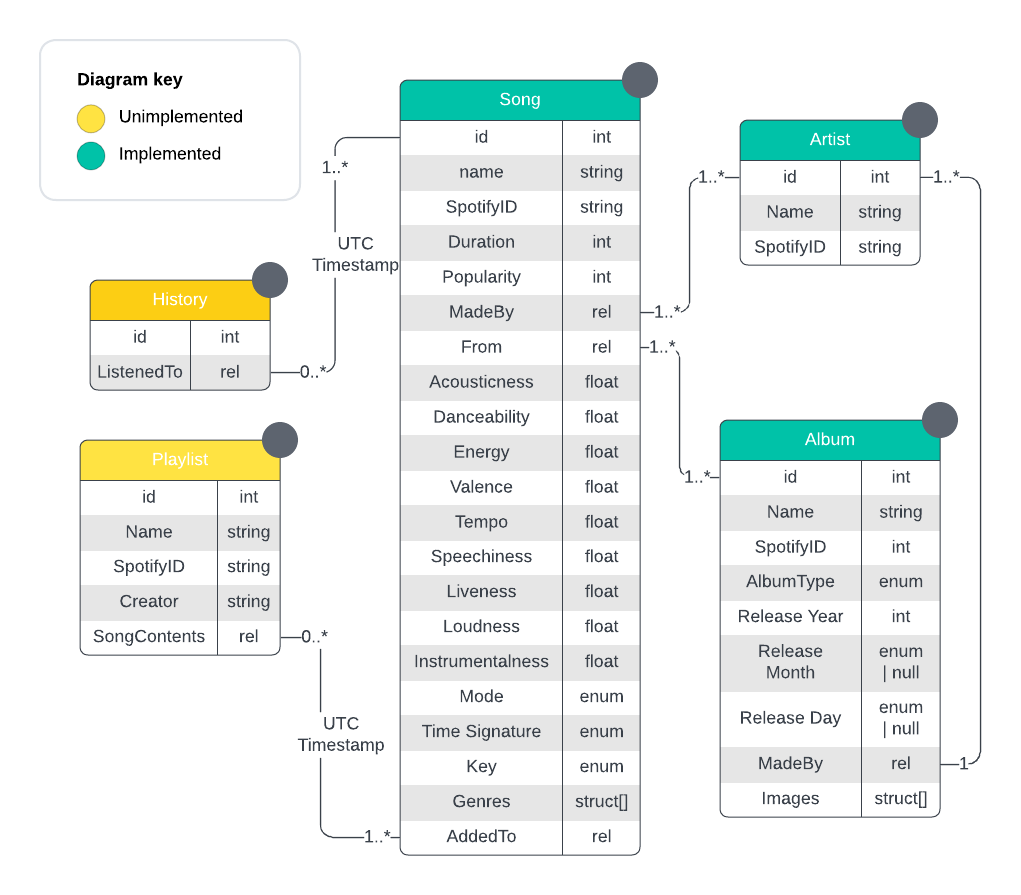
\includegraphics[angle=0, scale=0.85]{flecs_archetype_relationships_diagram.png}
    \caption{The Audyssey's Entities, Components and Relationships}
    \label{figure::archetype_relationship}
\end{figure}

\subsection{Echo Nest Attributes \& Spotify Metadata}%?How do I link these to the ECS components that I have mentioned before?
%TC: ignore
\begin{longtable}[c]{|c|p{14.5em}|c|p{5em}|p{5.5em}|}
    \caption{The Echo Nest Attributes \label{table::attributes}}\\%todo better caption
    \toprule
    \textbf{Attribute} & \textbf{Definition} & \textbf{Datatype} & \textbf{Possible Values} & \textbf{Continuous /Discrete} \\
    \midrule
    \endfirsthead

    \textbf{Acousticness} & A confidence measure of whether the track is acoustic. 1.0 represents high confidence the track is acoustic. & \texttt{float} & \texttt{0}-\texttt{1} & Continuous\\*
    \midrule
    \textbf{Danceability} & Describes how suitable a track is for     dancing based on a combination of musical elements including tempo, rhythm stability, beat strength, and verall regularity. A value of 1.0 is the most danceable. & \texttt{float} & \texttt{0}-\texttt{1} & Continuous\\*
    \cmidrule{1-4}
    \textbf{Energy} & Represents a perceptual measure of intensity and activity. Typically, energetic tracks feel fast, loud, and noisy. For example, death metal has high energy, while a Bach prelude scores low on the scale. Perceptual features contributing to this attribute include dynamic range, perceived loudness, timbre, onset rate, and general entropy.& \texttt{float} & \texttt{0}-\texttt{1} & Continuous\\*
    \midrule
    \textbf{Instrumentalness} & Predicts whether a track contains no vocals. ”Ooh” and ”aah” sounds are treated as instrumental in this context. Rap or spoken word tracks are clearly ”vocal”. The closer the instrumentalness value is to 1.0, the greater likelihood the track contains no vocal content. Values above 0.5 are intended to represent instrumental tracks, but confidence is higher as the value approaches 1.0.& \texttt{float} & \texttt{0}-\texttt{1} & Continuous \\*
    \midrule
    \textbf{Liveness} & Detects the presence of an audience in the recording. Higher liveness values represent an increased probability that the track was performed live. A value above 0.8 provides strong likelihood that the track is live.& \texttt{float} & \texttt{0}-\texttt{1} & Continuous\\*
    \cmidrule{1-5}
    \textbf{Loudness} & The overall loudness of a track in decibels (dB). Loudness values are averaged across the entire track and are useful for comparing relative loudness of tracks. Loudness is the quality of a sound that is the primary psychological correlate of physical strength (amplitude). Values typically range between -60 and 0 db. & \texttt{float} & \texttt{-60}-\texttt{0} & Continuous\\*
    \cmidrule{1-5}
    \textbf{Speechiness} & Speechiness detects the presence of spoken words in a track. The more exclusively speech-like the recording (e.g. talk show, audio book, poetry), the closer to 1.0 the attribute value. Values above 0.66 describe tracks that are probably made entirely of spoken words. Values between 0.33 and 0.66 describe tracks that may contain both music and speech, either in sections or layered, including such cases as rap music. Values below 0.33 most likely represent music and other non-speech-like tracks. & \texttt{float} & \texttt{0}-\texttt{1} & 
    \\*\cmidrule{1-5}
    \textbf{Valence} & A measure from 0.0 to 1.0 describing the musical positiveness conveyed by a track. Tracks with high valence sound more positive (e.g. happy, cheerful, euphoric), while tracks with low valence sound more negative (e.g. sad, depressed, angry). & \texttt{float} & \texttt{0}-\texttt{1} & Continuous\\*
    \midrule{1-5}
    \textbf{Tempo} & The overall estimated tempo of a track in beats per minute (BPM). In musical terminology, tempo is the speed or pace of a given piece and derives directly from the average beat duration. & \texttt{float} & \(\ge\)\texttt{0} & Continuous\\*
    \midrule
    \textbf{Key} & The key the track is in. Integers map to pitches using standard Pitch Class notation. E.g. 0 = C, and so on. If no key was detected, the value is -1. & \texttt{integer} & \texttt{None}/\texttt{C}/\texttt{C\#} /\texttt{D}/\texttt{D\#}/\texttt{E}/\texttt{F} /\texttt{F\#}/\texttt{G}/\texttt{G\#}/ \texttt{A}/\texttt{A\#}/\texttt{B} & \multirow{3}{*}{Discrete}\\*
    \cmidrule{1-4}
    \textbf{Mode} & Mode indicates the modality (major or minor) of a track, the type of scale from which its melodic content is derived. Major is represented by 1 and minor is 0. & \texttt{boolean} & \texttt{true}/\texttt{false} & \\*
    \cmidrule{1-4}
    \textbf{Time Signature} & An estimated time signature. The time signature (meter) is a notational convention to specify how many beats are in each bar (or measure). The time signature ranges from 3 to 7 indicating time signatures of "3/4", to "7/4". & \texttt{integer} & \texttt{3}/\texttt{4}/\texttt{5}/\texttt{6}/\texttt{7} & \\*
    \midrule
    
\end{longtable}
%TC: endignore

%TC: ignore
\begin{longtable}[c]{|c|p{7.5em}|p{7.5em}|p{5em}|p{5.5em}|}
    \caption{Spotify's Metadata \label{table::metadata}}\\%todo better caption
    \toprule
    \textbf{Metadata} & \textbf{Definition} & \textbf{Datatype} & \textbf{Possible Values} & \textbf{Continuous /Discrete} \\
    \midrule
    \endfirsthead

    \textbf{Title} & The full name of the track & \texttt{String} & Unicode & \multirow{4}{*}{Discrete} \\*
    \cmidrule{1-4}
    \textbf{Album} & What this track belongs to & \texttt{String} & Unicode & \\*
    \cmidrule{1-4}
    \textbf{Artist(s)} & The artist(s) that contributed to this track & \texttt{String[]} & Unicode & \\*
    \cmidrule{1-4}
    \textbf{Explicit} & Whether the track contains explicit words & \texttt{bool} & \texttt{true}/\texttt{false} & \\*
    \cmidrule{1-5}
    \textbf{Duration} & Length of the track (in ms) & \texttt{Integer} & \texttt{\(\ge\) 0} & \multirow{3}{*}{Continuous}\\*
    \cmidrule{1-4}
    \textbf{Popularity} & How 'popular' a track is, based on recent streams and other factors& \texttt{Integer} & \texttt{0-100} & \\*
    \cmidrule{1-4}
    \textbf{Added At} & UTC timestamp this track was added to a playlist & \texttt{String} & Unknown-Now&\\*
    \cmidrule{1-5}
    \textbf{Playlist(s)} & All (of a user's) playlists containing this song & \texttt{String[]} & Unicode & \multirow{2}{*}{Discrete}\\*
    \cmidrule{1-4}
    \textbf{Genre(s)} & List of genres and sub-genres & \texttt{root: String, sub: String[]} & Unknown &\\*
    \midrule
\end{longtable}
%TC: endignore

\section{Application State Flow}
\subsection{Spotify Authorisation}
To gain a user-specific API access token, Spotify's OAuth authorisation flow was implemented based on this \href{https://developer.spotify.com/documentation/web-api/tutorials/code-pkce-flow}{official guide}. This API token expires after an hour and requires sending another request to refresh this, however this mechanism was not implemented due to being needed. Once this access token has been retrieved and stored, the user's library can be loaded.

\subsection{Downloading User's Library (with Echo Nest Attributes)}
\subsubsection{SoundCharts API}
A full breakdown of this process can be found in \ref{appendix::Miro}, but here are the high-level steps:\begin{itemize}
    \item Request Spotify for all songs in a user's library
    \item Read serialized songs from a file into memory
    \item Fetch User's Spotify Library (only Liked Songs due to time constrains)
    \item Update songs missing attributes by requesting the SoundCharts API
\end{itemize}

\subsubsection{Exportify}
A full breakdown of this process can be found in \ref{appendix::Miro}, but here are the high-level steps:\begin{itemize}
    \item Login to \href{https://exportify.net/}{Exportify.net}
    \item Export a chosen playlist as a \texttt{.csv} file
    \item Convert the \texttt{csv} entries into flecs entities
    \item Fill missing fields (this was not implemented during this setup stage, but was done on-demand when a user clicked on a song)
\end{itemize}

\subsection{TODO: Main application yippee}
The \texttt{ViewSelector} UI component acts as the way to switch between views: Table, Static and Dynamic.
\begin{figure}[h]
    \centering
    
\includegraphics[scale=0.5]{app_view_selector.png}
    \caption{The UI Component for switching between views}
\end{figure}

\subsubsection{Table}
To make the development process easier, a library was used to implement the table UI: \href{https://www.ag-grid.com/react-data-grid/}{ag-grid}. This library was chosen due to its extensive feature set and easy assimilation into the existing codebase.
\begin{figure}[h]
    \centering
    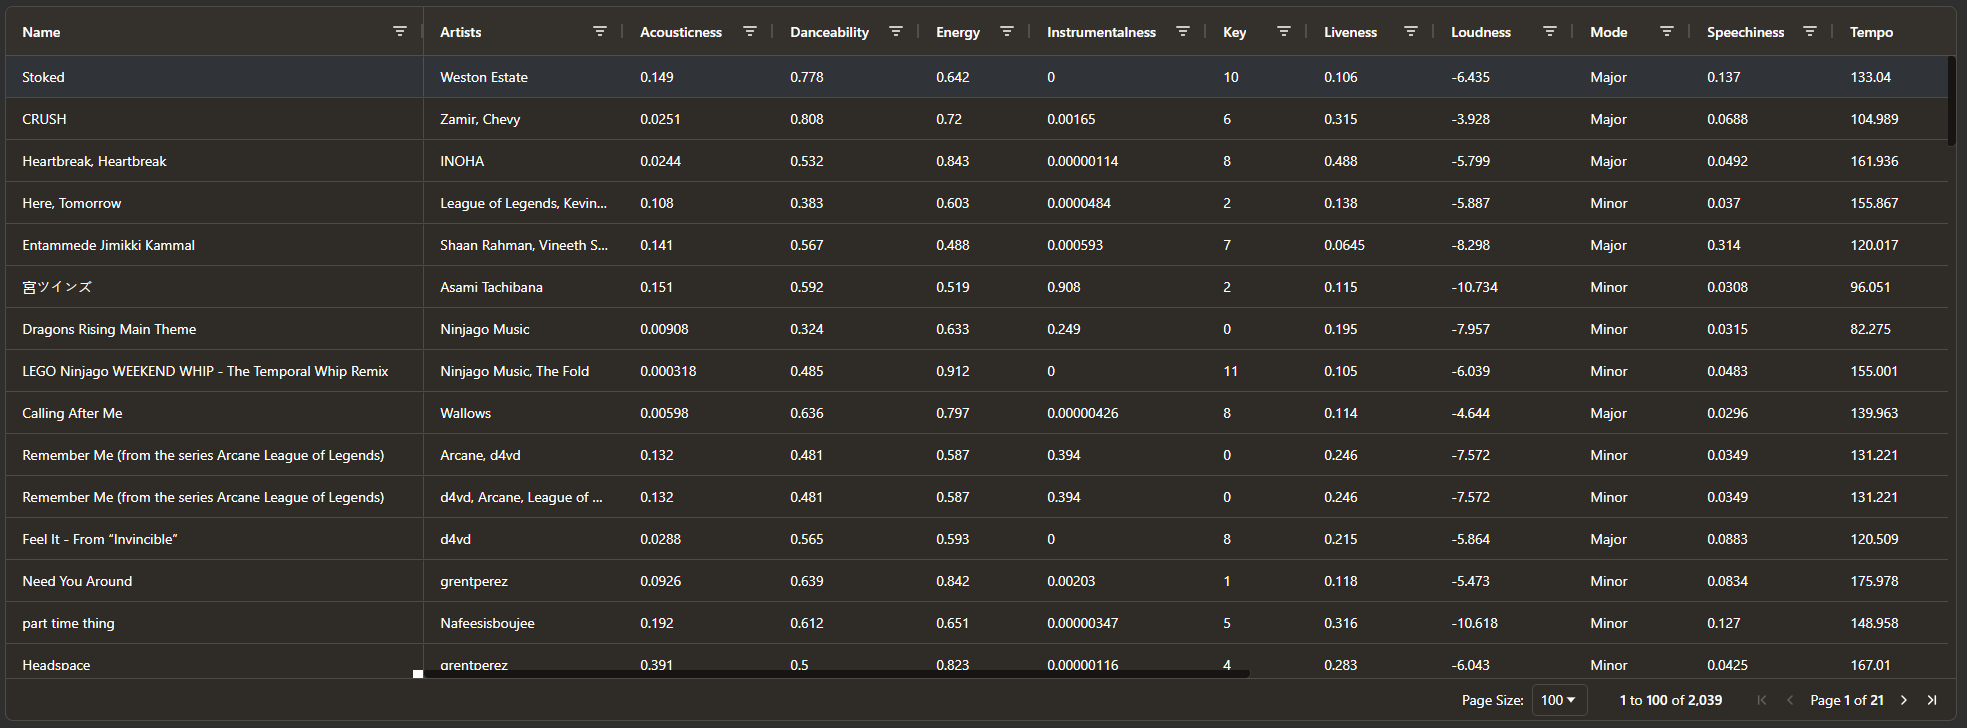
\includegraphics[scale=0.345]{app_table.png}
    \caption{Implementation of the Table View}
\end{figure}

\subsubsection{Static Graphs}%todo screenshots of the program
\paragraph{three.js Instanced Points}
Each song has their attribute values fetched based on the current attributes assigned to the axes. These values are then normalised and scaled to the size of the axis so that their spatial position directly represents their attribute values. The songs are represented by 3D spheres with an arbitrary colour. Their opacity is not 100\% to make it easier to see the density of songs.

\paragraph{Draggable Attribute Range Sliders}
These range sliders allow for zooming into the graph. Only the songs within the range of the left and right sliders are shown on the graph, as all other songs are greyed out and moved outside of the bounds of the axis. The sliders that are not attached to an axis can be dragged over to replace them: e.g. valence could be dragged to replace \_ in the y-axis slot.

Clicking any of the X, Y or Z buttons will result in that axis being turned off and and camera being locked to view the reamining two axes. If the Y-axis was turned off whilst the X-axis was inactive then the graph would switch to showing only the X and Z axes. Clicking an inactive axis will turn it back on, switching the graph view back to 3D.
\begin{figure}[h]
    \centering
    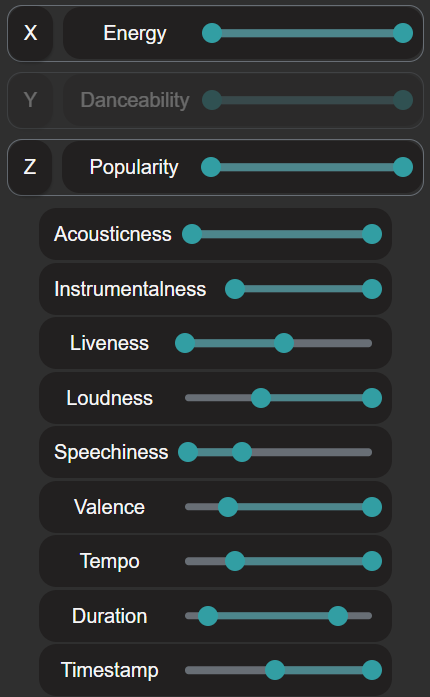
\includegraphics[scale=0.5]{app_attr_range_sliders.png}
    \caption{Implementation of the Draggable Attribute Range Sliders}
\end{figure}
\begin{figure}[h]
    \centering
    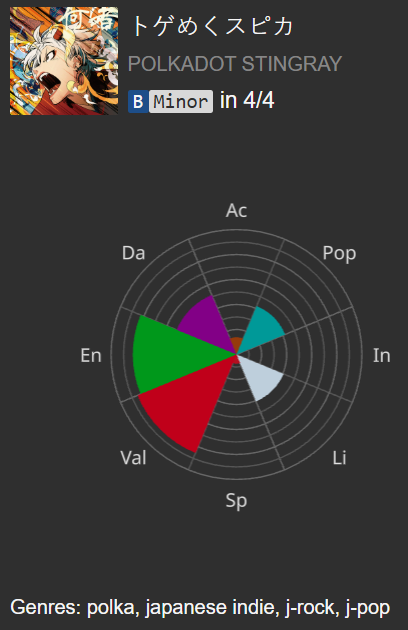
\includegraphics[scale=0.5]{app_detailed_song.png}
    \caption{Implementation of the Detailed Song Component}
\end{figure}

\paragraph{Detailed Song Component}
When a user clicks on a song sphere, a request is sent to the backend to get all the components for that song. These are then rendered as shown in figure \ref{}. The continuous metrics are rendered using a polar chart. Both key and mode have a specific colour background for each possible value.

\begin{figure}[h]
    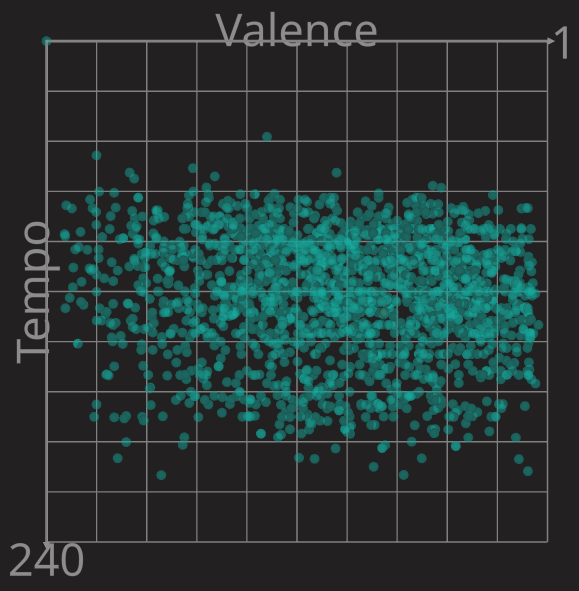
\includegraphics[scale=0.45]{final_static_2d.png}
    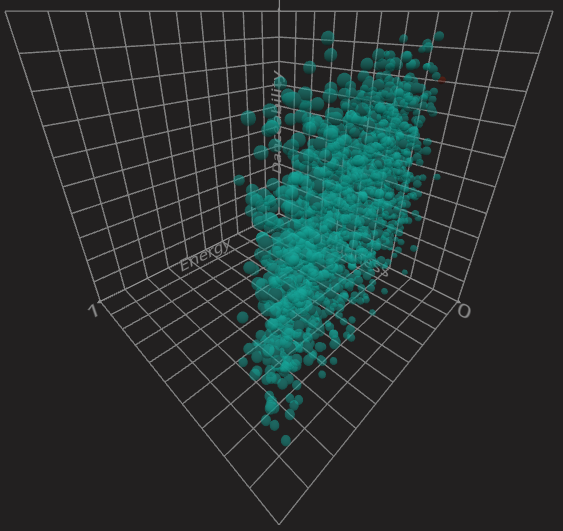
\includegraphics[scale=0.5]{final_static_3d.png}
    \caption{The Static Cartesian Graph implementation for 2 and 3 axes}
\end{figure}

\section{Development Methodology/Process}
%Wanted to be agile, actually was a waterful approach
A participatory approach was taken for the development process of this application (the Audyssey). Two music streaming service users who were asked help the development of the Audyssey as a review team (by acting as potential customers).

The chosen members also both represented both ends of the listening queue control spectrum. [Dhruv] is a fully active listener, they know the next song that they want to listen to, whereas [Josh] is significantly more passive, as they just pick a playlist and hit shuffle to always give them a randomly ordered queue.

\subsection{Design Review Meeting}
The initial design elements (including requirements, UI) were presented to the review team to get their feedback. Each requirement and its associated UI design were discussed with the team with any significant feedback noted down. The team were quite happy with the design resources, however they did have comments on reducing scope and new features.

\subsubsection{Reducing Scope}%todo reword/add more??
After discussing the requirements during the meeting, the key takeaway was that the core features and novel approachs were the graph views and as such these should be prioritised over the other requirements.

\subsubsection{Feature: Mixed Reality as a Medium for the Audyssey}
One proposed feature/future work by the review team was the adaptation of the 3D graph views to a mixed reality device. This would make the graphs "easier to navigate and explore" but would be a lot harder to develop. As such this feature was classified as out of scope but a good potential avenue for future work.

\subsubsection{Feature: Creating Playlists}
Similar to Organise Your Music, one member of of project noted that they would like the ability to create playlists by drawing a circle around a set of songs in the graph views. However, the main reason for this was so that they could easily re-listen to those songs again. As such this desire was adapted into a new requirement of being able to store and replay audio journeys.%! Remove this if it was already in the design section.
\paragraph{ReqID} Users \textbf{should} be able to listen to past audio journeys. %This is more difficult than it seems. How to show these when there's a lot of them. Finding the best way to store audio journeys requires a lot more research and investigation.

\subsection{Prototype Review Meeting}
As shown in the project plan, this meeting was planned to occur after an MVP was developed. This MVP would be showcased to the review team and any feedback would then be implemented in time for the final evaluation. Due to time constraints detailed in the Project Retrospective chapter, this meeting did not occur. As such, this feedback was instead discussed during the final evaluation itself. These design improvements are detailed in the Design Improvements section in the Evaluation Chapter.

%%% Talk about how I coded the project, being more pseudocodey, as in more alluding to how the code works, so it could be theoretically replicated in another language.